\section{Related Work}
\label{sec:related}
% ====================================================================

\paragraph{RL for legged locomotion.}
Modern quadruped controllers are typically learned via reinforcement
learning in simulation and transferred to real
hardware~\citep{hwangbo2019learning, rudin2022learning}.
\citet{chen2020learning} introduced the privileged
teacher--student paradigm, where a teacher with access to ground-truth
simulator state is distilled into a sensorimotor student.
\citet{lee2020learning} applied it to locomotion, training a student
from proprioceptive history alone and achieving sim-to-real
transfer on rough terrain.
\citet{kumar2021rma} introduced rapid motor adaptation, using a
learned module to estimate privileged parameters online.
\citet{miki2022learning} extended the framework to perceptive
locomotion with exteroceptive depth inputs.

\paragraph{Vision-based parkour.}
\citet{agarwal2023legged} introduced the scandot
representation for depth-based locomotion, distilling a
privileged teacher into a visual student.
Extreme Parkour~\citep{cheng2023parkour} and Robot Parkour
Learning~\citep{zhuang2023robot} build on this with CNN--GRU students
that process depth images, demonstrating climbing, jumping, and
crawling on real quadrupeds.
SoloParkour~\citep{chane2025soloparkour} replaces distillation with
off-policy RL warm-started from privileged experience, and
ANYmal Parkour~\citep{hoeller2024anymal} uses a hierarchical
skill-selection policy.
All five systems assume access to a depth camera at deployment.

\citet{jenkins2024learning} is the closest work to ours,
training an RGB parkour policy using visual domain randomization with a
fine-tuned MobileNetV2 backbone. In real-world trials, Jenkins
succeeded on hurdles but failed on gaps, suggesting that domain
randomization alone may not fully close the visual sim-to-real gap.

\paragraph{Sim-to-real for vision.}
Domain randomization~\citep{tobin2017domain} perturbs visual properties
(textures, lighting, colors) so the policy learns invariance through
exposure.
LucidSim~\citep{yu2024lucidsim} replaces randomization with
generative models that produce photorealistic training images.
\citet{xue2025opening} also uses photorealistic simulation for humanoid
loco-manipulation from RGB.
All three approaches require substantial rendering overhead.

\paragraph{Monocular depth estimation.}
MiDaS~\citep{ranftl2020towards} pioneered monocular
depth estimation.
Depth~Anything~V2 (DA2)~\citep{yang2024depth} achieves state-of-the-art
depth estimation using a vision transformer encoder trained
on 142M images, able to predict depth in meters.
Figure~\ref{fig:da2_qualitative}
shows example outputs.

\begin{figure}[htbp]
	\centering
	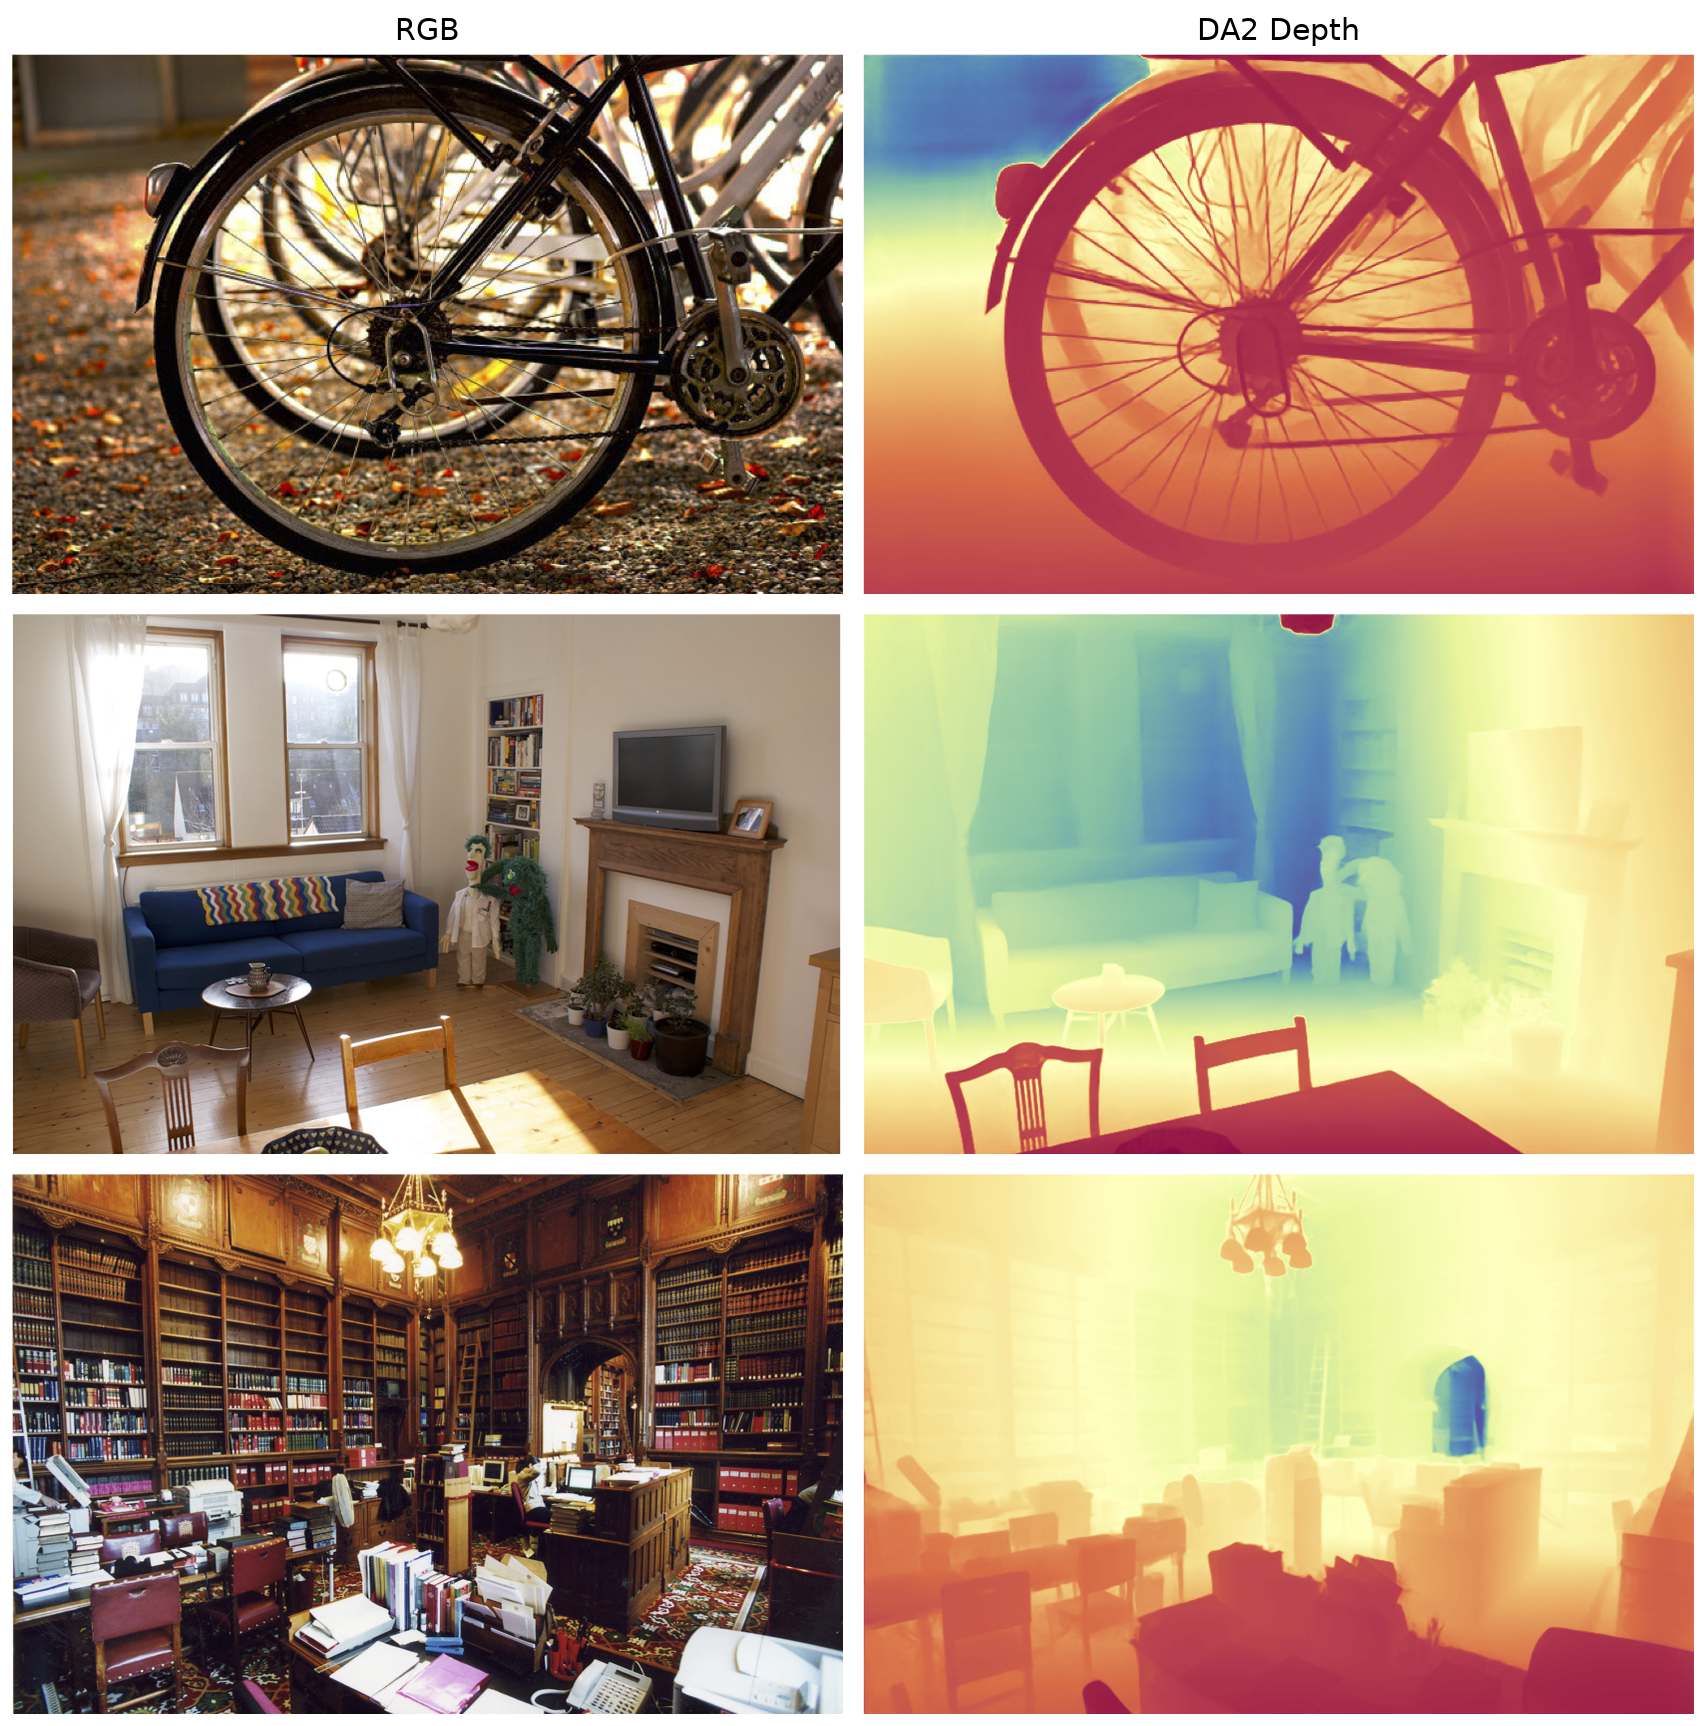
\includegraphics[width=\linewidth]{figures/depth_anything_v2_demo.png}
	\caption{Depth Anything V2 \cite{yang2024depth,depthanythingv2repo}.}
	\label{fig:da2_qualitative}
\end{figure}
